% Options for packages loaded elsewhere
\PassOptionsToPackage{unicode}{hyperref}
\PassOptionsToPackage{hyphens}{url}
%
\documentclass[
]{article}
\usepackage{lmodern}
\usepackage{amssymb,amsmath}
\usepackage{ifxetex,ifluatex}
\ifnum 0\ifxetex 1\fi\ifluatex 1\fi=0 % if pdftex
  \usepackage[T1]{fontenc}
  \usepackage[utf8]{inputenc}
  \usepackage{textcomp} % provide euro and other symbols
\else % if luatex or xetex
  \usepackage{unicode-math}
  \defaultfontfeatures{Scale=MatchLowercase}
  \defaultfontfeatures[\rmfamily]{Ligatures=TeX,Scale=1}
\fi
% Use upquote if available, for straight quotes in verbatim environments
\IfFileExists{upquote.sty}{\usepackage{upquote}}{}
\IfFileExists{microtype.sty}{% use microtype if available
  \usepackage[]{microtype}
  \UseMicrotypeSet[protrusion]{basicmath} % disable protrusion for tt fonts
}{}
\makeatletter
\@ifundefined{KOMAClassName}{% if non-KOMA class
  \IfFileExists{parskip.sty}{%
    \usepackage{parskip}
  }{% else
    \setlength{\parindent}{0pt}
    \setlength{\parskip}{6pt plus 2pt minus 1pt}}
}{% if KOMA class
  \KOMAoptions{parskip=half}}
\makeatother
\usepackage{xcolor}
\IfFileExists{xurl.sty}{\usepackage{xurl}}{} % add URL line breaks if available
\IfFileExists{bookmark.sty}{\usepackage{bookmark}}{\usepackage{hyperref}}
\hypersetup{
  pdftitle={Homework 1},
  pdfauthor={Jake Underland},
  hidelinks,
  pdfcreator={LaTeX via pandoc}}
\urlstyle{same} % disable monospaced font for URLs
\usepackage[margin=1in]{geometry}
\usepackage{color}
\usepackage{fancyvrb}
\newcommand{\VerbBar}{|}
\newcommand{\VERB}{\Verb[commandchars=\\\{\}]}
\DefineVerbatimEnvironment{Highlighting}{Verbatim}{commandchars=\\\{\}}
% Add ',fontsize=\small' for more characters per line
\usepackage{framed}
\definecolor{shadecolor}{RGB}{248,248,248}
\newenvironment{Shaded}{\begin{snugshade}}{\end{snugshade}}
\newcommand{\AlertTok}[1]{\textcolor[rgb]{0.94,0.16,0.16}{#1}}
\newcommand{\AnnotationTok}[1]{\textcolor[rgb]{0.56,0.35,0.01}{\textbf{\textit{#1}}}}
\newcommand{\AttributeTok}[1]{\textcolor[rgb]{0.77,0.63,0.00}{#1}}
\newcommand{\BaseNTok}[1]{\textcolor[rgb]{0.00,0.00,0.81}{#1}}
\newcommand{\BuiltInTok}[1]{#1}
\newcommand{\CharTok}[1]{\textcolor[rgb]{0.31,0.60,0.02}{#1}}
\newcommand{\CommentTok}[1]{\textcolor[rgb]{0.56,0.35,0.01}{\textit{#1}}}
\newcommand{\CommentVarTok}[1]{\textcolor[rgb]{0.56,0.35,0.01}{\textbf{\textit{#1}}}}
\newcommand{\ConstantTok}[1]{\textcolor[rgb]{0.00,0.00,0.00}{#1}}
\newcommand{\ControlFlowTok}[1]{\textcolor[rgb]{0.13,0.29,0.53}{\textbf{#1}}}
\newcommand{\DataTypeTok}[1]{\textcolor[rgb]{0.13,0.29,0.53}{#1}}
\newcommand{\DecValTok}[1]{\textcolor[rgb]{0.00,0.00,0.81}{#1}}
\newcommand{\DocumentationTok}[1]{\textcolor[rgb]{0.56,0.35,0.01}{\textbf{\textit{#1}}}}
\newcommand{\ErrorTok}[1]{\textcolor[rgb]{0.64,0.00,0.00}{\textbf{#1}}}
\newcommand{\ExtensionTok}[1]{#1}
\newcommand{\FloatTok}[1]{\textcolor[rgb]{0.00,0.00,0.81}{#1}}
\newcommand{\FunctionTok}[1]{\textcolor[rgb]{0.00,0.00,0.00}{#1}}
\newcommand{\ImportTok}[1]{#1}
\newcommand{\InformationTok}[1]{\textcolor[rgb]{0.56,0.35,0.01}{\textbf{\textit{#1}}}}
\newcommand{\KeywordTok}[1]{\textcolor[rgb]{0.13,0.29,0.53}{\textbf{#1}}}
\newcommand{\NormalTok}[1]{#1}
\newcommand{\OperatorTok}[1]{\textcolor[rgb]{0.81,0.36,0.00}{\textbf{#1}}}
\newcommand{\OtherTok}[1]{\textcolor[rgb]{0.56,0.35,0.01}{#1}}
\newcommand{\PreprocessorTok}[1]{\textcolor[rgb]{0.56,0.35,0.01}{\textit{#1}}}
\newcommand{\RegionMarkerTok}[1]{#1}
\newcommand{\SpecialCharTok}[1]{\textcolor[rgb]{0.00,0.00,0.00}{#1}}
\newcommand{\SpecialStringTok}[1]{\textcolor[rgb]{0.31,0.60,0.02}{#1}}
\newcommand{\StringTok}[1]{\textcolor[rgb]{0.31,0.60,0.02}{#1}}
\newcommand{\VariableTok}[1]{\textcolor[rgb]{0.00,0.00,0.00}{#1}}
\newcommand{\VerbatimStringTok}[1]{\textcolor[rgb]{0.31,0.60,0.02}{#1}}
\newcommand{\WarningTok}[1]{\textcolor[rgb]{0.56,0.35,0.01}{\textbf{\textit{#1}}}}
\usepackage{graphicx,grffile}
\makeatletter
\def\maxwidth{\ifdim\Gin@nat@width>\linewidth\linewidth\else\Gin@nat@width\fi}
\def\maxheight{\ifdim\Gin@nat@height>\textheight\textheight\else\Gin@nat@height\fi}
\makeatother
% Scale images if necessary, so that they will not overflow the page
% margins by default, and it is still possible to overwrite the defaults
% using explicit options in \includegraphics[width, height, ...]{}
\setkeys{Gin}{width=\maxwidth,height=\maxheight,keepaspectratio}
% Set default figure placement to htbp
\makeatletter
\def\fps@figure{htbp}
\makeatother
\setlength{\emergencystretch}{3em} % prevent overfull lines
\providecommand{\tightlist}{%
  \setlength{\itemsep}{0pt}\setlength{\parskip}{0pt}}
\setcounter{secnumdepth}{-\maxdimen} % remove section numbering
\usepackage{amsmath}
\usepackage{dcolumn}
\usepackage{rotating}
\usepackage{amsmath}
\usepackage{dcolumn}
\usepackage{rotating}

\title{Homework 1}
\usepackage{etoolbox}
\makeatletter
\providecommand{\subtitle}[1]{% add subtitle to \maketitle
  \apptocmd{\@title}{\par {\large #1 \par}}{}{}
}
\makeatother
\subtitle{ECON 24450 Spring, 2021}
\author{Jake Underland}
\date{2021-04-27}

\begin{document}
\maketitle

{
\setcounter{tocdepth}{2}
\tableofcontents
}
\newcommand{\argmax}{\mathop{\mathrm{argmax}}}

\hypertarget{model-of-adverse-selection}{%
\section{1. Model of Adverse
Selection}\label{model-of-adverse-selection}}

\textit{Consider the following adverse selection model based on Einav and Finkelstein (2011). Suppose an agent has income $I$ and experiences a loss of $L$ with probability $\theta$. The agent can purchase full insurance in a competitive market for an amount $p$. The agent has a utility function $u$ ($u' > 0, u'' < 0$).}.

\hypertarget{a.}{%
\subsection{a.}\label{a.}}

\textit{Write down the condition for whether the individual insures. Solve for $\theta$ and interpret your result.}

Assuming \(p, L>0\), \[\begin{aligned}
\underbrace{u(I-p)}_{\text{Expected utility of being insured}} &\geq \underbrace{\theta u(I-L) + (1 - \theta)u(I)}_{\text{Expected utility of no insurance}} \\ 
\implies \theta ^ * &\geq \frac{u(I) - u(I-p)}{u(I) - u(I-L)}
\end{aligned}\] The above shows that the smaller the utility of being
uninsured in a bad state is relative to the utility of being insured and
paying for insurance, the lower the threshold for \(\theta\) to get
insurance. Or, those who face higher costs in an adverse event are more
likely to select into insurace (adverse selection).

\hypertarget{b.}{%
\subsection{b.}\label{b.}}

\textit{Suppose that the distribution of $\theta$ in the economy is given by the cdf $F(\theta)$. Write down how the competitive insurance company will set the price $p$ in terms of $\theta$. You do not need to solve explicitly for the equilibrium $p$.}

From competition, prices will be actuarially fair.
\[ p = E[\text{Costs}]\]
\[\text{Costs} = \begin{cases} \theta L \dots \theta \geq \theta ^ * \\
0 \dots \theta < \theta ^ * \end{cases}\] \[\begin{aligned} 
\implies p &= E[\theta L | \theta \geq \theta ^*] P( \theta \geq \theta ^ *) + E[0]P(\theta < \theta ^ *) \\
 &= E[\theta L|\theta \geq \theta ^ *] P(1 - F(\theta ^ *)
\end{aligned}\]

\hypertarget{c.}{%
\subsection{c.~}\label{c.}}

\textit{Show graphically the AC, MC, and demand curves, and characterize the efficient outcome and equilibrium outcome for insurance coverage in the following cases:}

\hypertarget{i.}{%
\subsubsection{i.}\label{i.}}

\textit{There is adverse selection and demand is everywhere above marginal cost.}

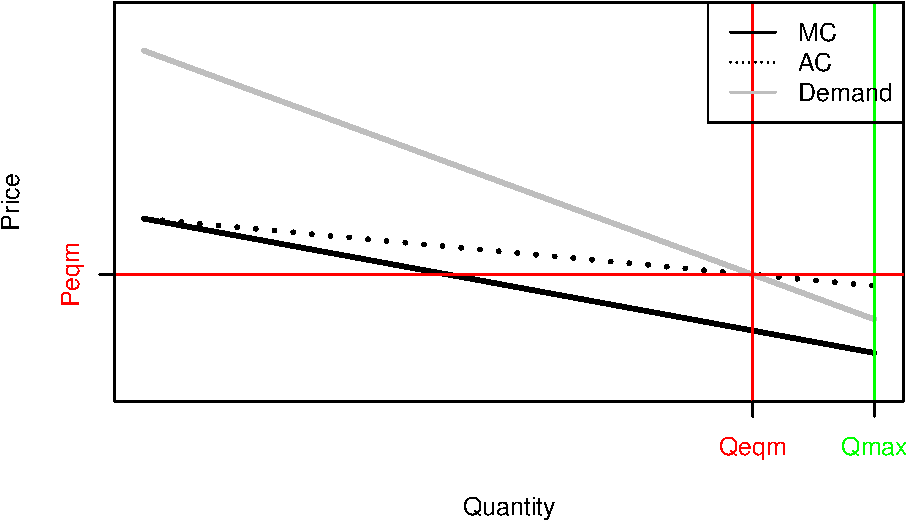
\includegraphics{Pset1_files/figure-latex/unnamed-chunk-2-1.pdf}

The efficient outcome is Qmax, shown in green above, since at all points
of the graph demand outweighs marginal cost. However, the equilibrium is
characterized by the break-even point, where average cost and demand
intersect, and is shown in red as Qeqm and Peqm in the graph.

\hypertarget{ii.}{%
\subsubsection{ii.}\label{ii.}}

\textit{There is adverse selection and demand is everywhere above average cost.}

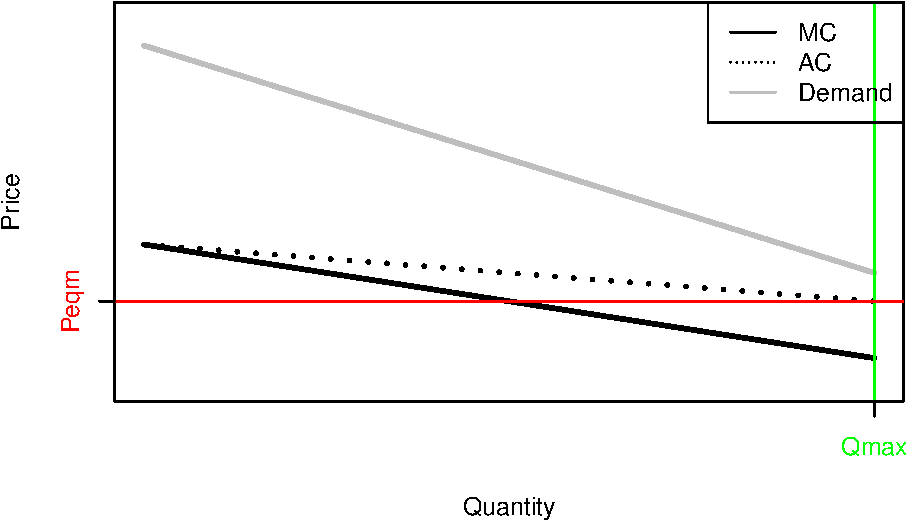
\includegraphics{Pset1_files/figure-latex/unnamed-chunk-3-1.pdf}

In the above, the efficient outcome Qmax is provided at equilibrium at
price Peqm, since that is the break-even point at which competitive
firms will provide insurance. Because demand is above average cost
everywhere, firms can provide Qmax without lowering their profit below
0.

\hypertarget{iii.}{%
\subsubsection{iii.}\label{iii.}}

\textit{There is adverse selection and demand is everywhere above MC and everywhere below AC.}

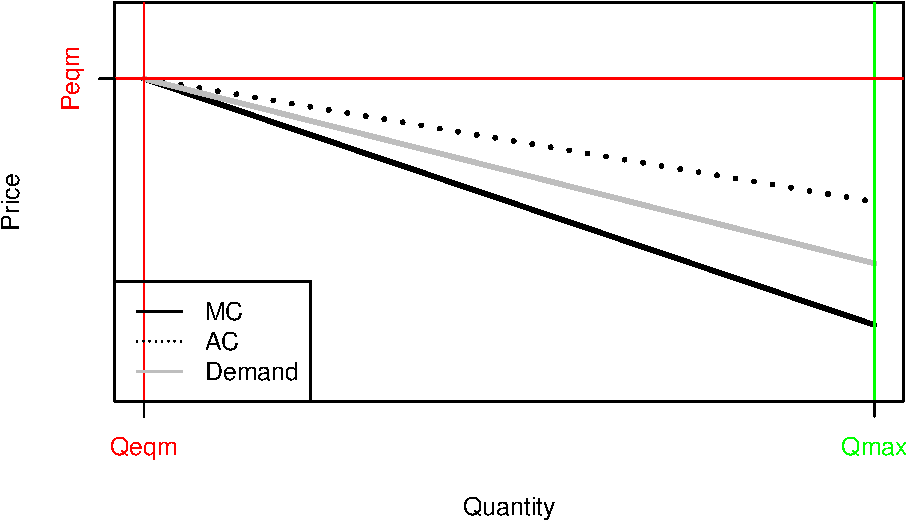
\includegraphics{Pset1_files/figure-latex/unnamed-chunk-4-1.pdf}

The above graph shows a case of complete unraveling. Because the MC
curve is always below the demand curve, the efficient outcome is Qmax.
However, the AC curve lies above the demand curve everywhere on the
graph, making provision of insurance infeasible for firms (since it
would yield negative profits). Thus, at equilibrium, firms will provide
no insurance.

\hypertarget{iv.}{%
\subsubsection{iv.}\label{iv.}}

\textit{There is advantageous selection (i.e., those with highest demand have the lowest $\theta$). Why
might such a situation arise?}

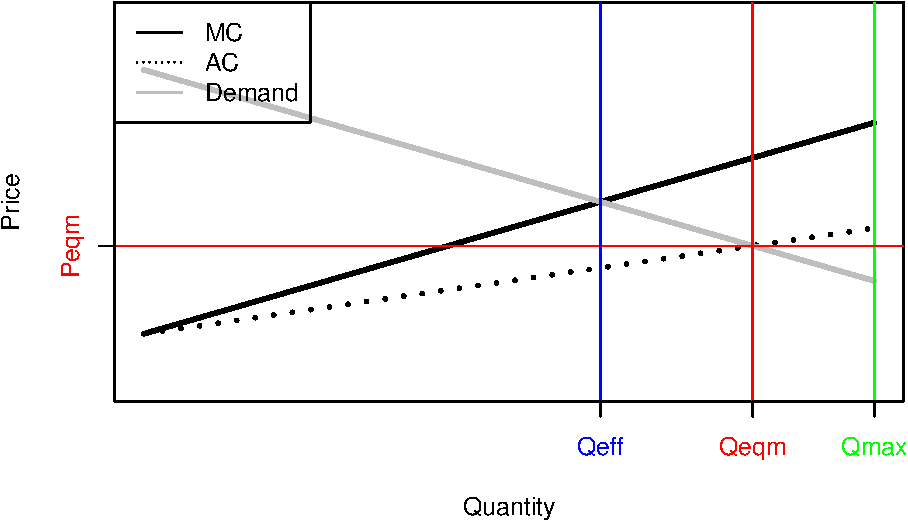
\includegraphics{Pset1_files/figure-latex/unnamed-chunk-5-1.pdf}

With advantageous selection, the higher risk people carry, the less risk
averse they are, and vice-versa, leading to an upward sloping MC curve.
This is situation is possible in markets where higher risk aversion
leads to choices in the consumer's daily life that lower their risk. For
example, those with higher risk aversion in terms of their health are
more likely to eat healthy, exercise, and lead a healthier lifestyle.
This in turn may lower their risk of health problems and lower the
firm's expected cost of insuring these individuals, leading to
advantageous selection. In this market, the equilibrium is defined by
the same condition as adverse selection, namely AC = Demand. However,
this would lead to overinsurance of individuals whose demand outweighs
the marginal cost of insuring them, leading to societal losses. In this
case, the efficient outcome is for firms to provide Qeff, shown in blue,
in accordance with the principles of usual supply and demand analysis
without private information and adverse selection.

\hypertarget{adverse-selection}{%
\section{2. Adverse Selection}\label{adverse-selection}}

\textit{The likelihood of getting breast cancer is determined by a combination of family history and lifestyle choices, especially smoking. Suppose the probability of getting cancer breaks down as follows:}

\begin{tabular}{ l c r }
\text{ } & \text{Smoker} & \text{Non-smoker} \\
\text{Good history} & 10\% & 5 \% \\
\text{Bad history} & 20 \% & 10 \%
\end{tabular}

\textit{The expected cost for treating breast cancer is $\$10,000$. Assume that in addition to the expected dollar value of the policy, all women (no matter their risk) value the security of having insurance for breast cancer for an additional $\$400$. Assume that $25\%$ of women fall into each category.}

\hypertarget{a.-1}{%
\subsection{a.}\label{a.-1}}

\textit{Suppose the insurance company cannot observe either smoking status or family history and offers the same insurance policy to all individuals. What price would it have to charge to break even if everyone participated in the insurance market? At the break-even price, which women would participate in the market? (Don’t forget the risk premium.) Relate your answer to adverse selection.}

A competitive firm would charge the expected cost of insurance given the
distribution of the population and the risks of breast cancer (i.e.,
risk of collecting insurance). If the firm cannot observe the different
populations, then the expected cost would be:

\begin{Shaded}
\begin{Highlighting}[]
\CommentTok{# Expected cost of insurance}
\FloatTok{0.25} \OperatorTok{*}\StringTok{ }\FloatTok{0.1} \OperatorTok{*}\StringTok{ }\DecValTok{10000} \OperatorTok{+}\StringTok{ }\FloatTok{0.25} \OperatorTok{*}\StringTok{ }\FloatTok{0.05} \OperatorTok{*}\StringTok{ }\DecValTok{10000} \OperatorTok{+}\StringTok{ }\FloatTok{0.25} \OperatorTok{*}\StringTok{ }\FloatTok{0.2} \OperatorTok{*}\StringTok{ }\DecValTok{10000} \OperatorTok{+}\StringTok{ }\FloatTok{0.25} \OperatorTok{*}\StringTok{ }\FloatTok{0.1} \OperatorTok{*}\StringTok{ }\DecValTok{10000}
\end{Highlighting}
\end{Shaded}

\begin{verbatim}
## [1] 1125
\end{verbatim}

Thus, the price would be \(p = 1125\). Then, each population renders
insurance a value equivalent to their expected risk plus \(\$400\),
which is their risk premium. Thus, each population's value of insurance
is as follows:

\begin{tabular}{ l c r }
\text{ } & \text{Smoker} & \text{Non-smoker} \\
\text{Good history} & \$1400 & \$900  \\
\text{Bad history} &  \$2400 & \$1400
\end{tabular}

From here we can easily see that all populations except for Non-smokers
with a good family history will buy insurance. This is adverse
selection, as only those with a certain level of risk select into
insurance, but since information about risk is private, the firm cannot
price discriminate and capture all demand.

\hypertarget{b.-1}{%
\subsection{b.}\label{b.-1}}

\textit{Suppose the insurance company can observe whether an individual is a smoker and is allowed to price separately for smokers and non- smokers. Is there a price at which the insurer could make a profit and provide insurance for all smokers? Is there a price at which the insurer could make a profit and provide insurance for all non-smokers?}

\begin{Shaded}
\begin{Highlighting}[]
\CommentTok{# Expected cost of insurance for smokers}
\FloatTok{0.5} \OperatorTok{*}\StringTok{ }\FloatTok{0.1} \OperatorTok{*}\StringTok{ }\DecValTok{10000} \OperatorTok{+}\StringTok{ }\FloatTok{0.5} \OperatorTok{*}\StringTok{ }\FloatTok{0.2} \OperatorTok{*}\StringTok{ }\DecValTok{10000} 
\end{Highlighting}
\end{Shaded}

\begin{verbatim}
## [1] 1500
\end{verbatim}

\begin{Shaded}
\begin{Highlighting}[]
\CommentTok{# Expected cost of insurance for non-smokers}
\FloatTok{0.5} \OperatorTok{*}\StringTok{ }\FloatTok{0.05} \OperatorTok{*}\StringTok{ }\DecValTok{10000} \OperatorTok{+}\StringTok{ }\FloatTok{0.5} \OperatorTok{*}\StringTok{ }\FloatTok{0.1} \OperatorTok{*}\StringTok{ }\DecValTok{10000}
\end{Highlighting}
\end{Shaded}

\begin{verbatim}
## [1] 750
\end{verbatim}

Thus, in order for the firm to make a positive profit, it must price
\(p>1500\) for smokers and \(p>750\) for non-smokers. Since smokers with
a good family history value insurance at \(\$1400\), there is no price
at which firms can capture the demand of these women without making
negative profit. Thus, there is no price at which the insurer can make a
profit and provide insurance for all smokers. Non-smokers, on the other
hand, both value insurance at above \(\$750\), the expected cost of
insuring non-smokers. Thus, any price \(\$750 < p < \$900\) will give
the firm positive profit and capture all demand of non-smokers.

\hypertarget{c.-1}{%
\subsection{c.~}\label{c.-1}}

\textit{Given your answer to (b), if the insurer cannot serve all of the individuals in one of the smoking categories, what price must it charge to break-even while serving only the individuals with the “bad” family history in that smoking category?}

The firm must charge the expected cost of ensuring the smokers with bad
family history, given below.

\begin{Shaded}
\begin{Highlighting}[]
\CommentTok{# Expected cost of insuring smokers with bad history (dollars)}
\FloatTok{0.2} \OperatorTok{*}\StringTok{ }\DecValTok{10000}
\end{Highlighting}
\end{Shaded}

\begin{verbatim}
## [1] 2000
\end{verbatim}

\hypertarget{d.}{%
\subsection{d.~}\label{d.}}

\textit{Given your answers to (b) and (c), when the insurance company can discriminate on the basis of smoking behavior, what is the difference between the break-even prices offered to smokers vs. non-smokers? Which women participate in the insurance market in this case? Which groups are made better off or worse off than in the case with a single policy from part (a)?}

For smokers, the firm will charge the break-even price of \(\$2000\),
thus driving smokers with good family history out of the insurance
market. For non-smokers, the firm will charge the break-even price of
\(\$750\), in which case both types of non-smokers will buy insurance.\\
Both categories of smokers will be made worse off from discrimination.
For those with good family history, under (a) they would have a
\(\$275\) surplus of utility since they value insurance at \(\$1400\)
and purchase at the break-even price of \(\$1125\), but under (b) they
would have no insurance. For those with a bad family history, under (a)
they would have a surplus of \(\$2400 - \$1125 = \$1275\), but under (b)
their surplus will be the risk premium of \(\$400\) since the firm will
charge the break-even price for insuring at their risk-level.\\
Non-smokers, on the other hand, will be better off than under (a). Under
(a), non-smokers with good family history will incur a loss by buying
insurance (\(\$900 - \$1125 = -\$225\)), but under (b), they would have
a surplus of \(\$900 - \$750 = \$ 150\). Likewise, non-smokers with bad
family history will have a surplus \(\$1400 - \$750 = \$650\) under (b)
as opposed to \(\$1400 - \$1125=\$275\) under (a).

\hypertarget{unemployment-insurance}{%
\section{3. Unemployment insurance}\label{unemployment-insurance}}

\textit{Ron Swanson works at a steel mill, and earns an amount $E$. He faces some risk of being unemployed, denoted by $p$. If he becomes unemployed, he loses all of his income. His utility is of the form $U = ln(C)$, where $C$ is consumption and is equal to income.}

\hypertarget{a.-2}{%
\subsection{a.}\label{a.-2}}

\textit{Suppose initially that there is no public unemployment insurance, but there is a well-functioning private unemployment insurance market. In this market, you pay a premium ($a$) if you are employed, and in return you get some net benefits if unemployed ($b$). Suppose that the private unemployment insurance is actuarially fair (so that insurer makes zero expected profits on Ron). Ron is deciding how much insurance to buy, or how much income he will have if he is employed next period and how much he will have if he is unemployed next period. Derive mathematically how much insurance Ron will buy. Show whether this is more or less than full insurance.}

2 steps towards derivation:
\[\begin{cases} 1. \text{Break-even budget constraint} \\
 2. \text{Ron's decision} \end{cases}\]\\

\begin{enumerate} 
\item 
$$\begin{aligned} 
\underbrace{(1-p)a}_{\text{Expected revenue}} &= \underbrace{pb}_{\text{Expected cost}} \\
\implies b^ * &= \frac{1-p}{p}a
\end{aligned}$$ 

\item 
$$\begin{aligned}
&\max_{a, b} \{ p\ln (b) + (1-p) \ln (E-a) \text{ s.t. } b = \frac{1-p}{p}a \} \\
\implies & \max_{a, b} \mathcal{L} = p\ln (b) + (1-p) \ln (E-a) + \lambda [\frac{1-p}{p}a - b]
\end{aligned}$$  
FOCs: 
$$\begin{aligned}
&[b] \text{ }\space \frac{p}{b} = \lambda \\
&[a] \text{ }\space -\frac{1-p}{E-a} = -\frac{1-p}{p}\lambda \\
&[\lambda ] \text{ }\space b = \frac{1-p}{p}a
\end{aligned}$$
Solving this for $a, b$, we get 
$$a = Ep, \space b = E(1-p)$$
\end{enumerate}

Comparing consumption levels at both periods, we see that when
unemployed consumption is \[C = b = E(1-p)\] whereas when employed,
consumption is \[C = E - a = E(1-p)\] Thus, the above private insurance
is equivalent to full insurance.

\hypertarget{b.-2}{%
\subsection{b.}\label{b.-2}}

\textit{Continue to assume that the private insurance is actuarially fair. Now the government introduces a public insurance system. The system replaces half of Ron’s lost earnings ($E/2$) if he becomes unemployed. It is financed by an actuarially fair tax on Ron if Ron is employed—so the government expects to break even on this insurance policy. Now how much private insurance will Ron want? How does it relate to part (a)? Why? (The algebra is kind of a mess, but Ron would say that it builds character.)}

3 steps towards derivation:
\[\begin{cases} 1. \text{Break-even budget constraint of private insurance} \\
3. \text{Break-even budget constraint of public insurance} \\
 2. \text{Ron's decision} \end{cases}\]

\begin{enumerate} 
\item 
From (a), 
$$\begin{aligned} 
b^ * &= \frac{1-p}{p}a
\end{aligned}$$ 

\item
$$\begin{aligned} 
\underbrace{p\frac{E}{2}}_{\text{Expected revenue}} &= \underbrace{(1-p)t}_{\text{Expected cost}} \\
\implies t^ * &= \frac{pE}{2(1-p)}
\end{aligned}$$

\item 
$$\begin{aligned}
&\max_{a, b, t} \{ p\ln (b + \frac{E}{2}) + (1-p) \ln (E-a-t) \space \text{  s.t.  } \space b = \frac{1-p}{p}a, \space t = \frac{pE}{2(1-p)} \} \\
\implies & \max_{a, b, t} \mathcal{L}= p\ln (b + \frac{E}{2}) + (1-p) \ln (E-a-t) +  \lambda_p [\frac{1-p}{p}a - b] + \lambda_g[\frac{pE}{2(1-p)} - t]
\end{aligned}$$  
FOCs: 
$$\begin{aligned}
&[b] \space \text{ } \frac{p}{b+\frac{E}{2}} = \lambda _p\\
&[a] \space \text{ }-\frac{1-p}{E-a -t} = -\frac{1-p}{p}\lambda _p \\
&[t]\space \text{ }-\frac{1-p}{E-a -t} = -\lambda_g \\
&[\lambda_p ] \text{ }\space b = \frac{1-p}{p}a \\
&[\lambda_g] \text{ }\space t = \frac{pE}{2(1-p)}
\end{aligned}$$
Using $[b], [a]$ we get  
$$b + \frac{E}{2} = E - a - t$$
Plug $[\lambda_p ], [\lambda_g]$ and simplify to yield
$$\begin{aligned} 
a^ * &= \frac{Ep(1-2p)}{2(1-p)} \\
b ^* &= \frac{E(1-2p)}{2} \\
t ^ * &= \frac{pE}{2(1-p)}
\end{aligned}$$

\end{enumerate}

Observe that\\
\[\begin{aligned}
E - a - t = E - \frac{Ep(1-2p)}{2(1-p)} -\frac{pE}{2(1-p)} &= E(1-p) \\
 b +  \frac{E}{2} = \frac{E(1-2p)}{2} + \frac{E}{2} &= E(1-p)
\end{aligned} \] From here, we can deduce that Ron is merely
supplementing his government insurance with private insurance in order
to achieve full insurance derived in (a).

\hypertarget{c.-2}{%
\subsection{c.~}\label{c.-2}}

\textit{What is the effect of providing this public unemployment insurance on Ron’s well-being (as measured by expected utility)?}

From (b), since we know under either scenario, full insurance is
achieved and consumption in the two periods for both situations are the
same, there is no effect on Ron's expected utility (although Ron Swanson
would likely prefer the situation in (a) considering his intense hatred
of government intervention).

\hypertarget{d.-1}{%
\subsection{d.~}\label{d.-1}}

\textit{Now suppose that there is no private unemployment insurance at all. In this world, calculate the effect on Ron’s well-being of introducing actuarially fair public unemployment insurance that replaces half of his lost income. Is this gain larger or smaller than in (c)?}

Ron's expected utility with government insurance:
\[E[u] = p\ln(\frac{E}{2}) + (1-p)\ln(E-\frac{pE}{2(1-p)})\] Ron's
expected utility without any insurance:\\
\[E[u] = p\ln(0) + (1-p)\ln(E) = -\infty p + (1-p)\ln(E) \approx -\infty\]
Thus, Ron's expected utility experiences a significantly large gain from
the introduction of an actuarially fair government insurance. This gain
is much larger than the gain (or lack thereof) observed in (c).

\hypertarget{e.}{%
\subsection{e.}\label{e.}}

\textit{Is the analysis of (c) or (d) more applicable to US unemployment insurance and why? What is the empirical evidence on how public unemployment insurance affects well-being? What is the empirical evidence on the costs of public unemployment insurance and does this question consider them?}

The situation in (d) since private unemployment insurance does not exist
in the US, ostensibly due to private information, adverse selection and
complications resulting from moral hazard. Gruber (1997) finds evidence
that the consumption smoothing effects of unemployment insurance are
nontrivial and thus improve the well being of individuals. The empirical
evidence on the costs of public unemployment insurance, summarized in
Krueger \& Meyers (2002), indicate that these programs tend to increase
the duration of unemployment in workers at greater levels than usual
responses to wages and taxes. This implies that there may be a moral
hazard problem to be considered in UI, and other distortionary costs
which this question does not consider.

\hypertarget{risk-aversion-moral-hazard}{%
\section{4. Risk aversion: moral
hazard}\label{risk-aversion-moral-hazard}}

\textit{Jean-Ralphio can exert effort ($e = 1$) to avoid an accident at work or not exert any effort ($e = 0$). If $e = 1$, the probability of an accident is $1/2$. If $e = 0$, the probability of
an accident is $1$. Jean-Ralphio’s income without the accident is $\$100$. In case of an accident, medical
expenses will be $\$64$, so his net income in that case is $\$36$. Jean-Ralphio’s utility of income is $\sqrt{I}$. The cost of effort, $C(e)$, is $0$ if effort is $e = 0$ and $1$ if effort is $e = 1$. Jean-Ralphio’s utility function is
$u(I,e)= \sqrt{I}−C(e)$.}

\hypertarget{a.-3}{%
\subsection{a.}\label{a.-3}}

\textit{Is Jean-Ralphio risk averse, risk neutral, or risk loving? Explain algebraically. Consider a world without insurance in which Jean-Ralphio, uncharacteristically, exerts effort. Calculate the certainty equivalent and risk premium associated with the risk of getting injured and explain what each term means in words.}

Jean-Ralphio is risk averse:\\
\[\begin{aligned} 
u(I, e) &= \sqrt{I} - C(e) \\
\frac{\partial}{\partial I} u(I, e) &= \frac{1}{2\sqrt{I}} > 0 \\
\frac{\partial^2}{\partial I^2} u(I, e) &= -\frac{1}{4}I^{-\frac{3}{2}} < 0
\end{aligned}\] Because \(u' > 0\) and \(u'' <0\), we know that JR's
utility function is concave and thus he is risk averse.\\
Conditioning on JR exerting effort \(e=1\), his income is
\[\begin{aligned}
I_0 &= \$100 \\
I_A &= \$36
\end{aligned}\] Thus, his expected income is:
\[\frac{1}{2} \$100 + \frac{1}{2} \$36 = \$ 68\] The utility of this
uncertain expectation is in turn:
\[E[u|e=1] = \frac{1}{2} (\sqrt{100} - 1) + \frac{1}{2} (\sqrt{36} - 1)]= 7\]
The certainty equivalent is the dollar amount of certain income that
brings him an equal amount of utility, 7. \[\begin{aligned} 
\sqrt{x} - 1 &= 7 \\
\implies \sqrt{x} &= 8 \\
\implies x &= 64
\end{aligned}\]

Thus, JR's certainty equivalent is \(\$ 64\). From here, his risk
premium is \[\$68 - \$64 = \$4\]

\hypertarget{b.-3}{%
\subsection{b.}\label{b.-3}}

\textit{Compare Jean-Ralphio’s expected utility when he exerts effort versus when he doesn’t. Will Jean-Ralphio choose to exert effort?}

\[\begin{aligned} 
E[u|e=1] = 7 > 6 = \sqrt{36} =  E[u|e=0]
\end{aligned}\] Thus, JR uncharacteristically decides to exert effort.

\hypertarget{c.-3}{%
\subsection{c.~}\label{c.-3}}

\textit{Now suppose there is a risk neutral insurance company. Suppose the insurance company cannot monitor Jean-Ralphio’s behavior. The insurance company considers three contracts, labeled A, B, and C. Each contract specifies the price $p$ and the amount of money $d$ Jean-Ralphio gets in case of an accident. Given $p$ and $d$, Jean-Ralphio’s final income in case of no accident is $I_0 = 100 − p$ and his final income in case of an accident is $I_A = 36 − p + d$. The contracts are as follows:}

\begin{tabular}{ l c r } 
\text{Contract} & \text{Price} $p$ & \text{Payment} $d$ \\
\text{A} & \$36 & \$64 \\
\text{B} & \$19 & \$47 \\
\text{C} & \$19 & \$32 
\end{tabular}

\textit{For each of the two contracts, calculate his final incomes, $I_0$ and $I_A$, in the two outcomes, and list them in a table. Which of these contracts offers full insurance to JR?}

\begin{tabular}{ l c r } 
\text{Contract} & $I_0$ & $I_A$\\
\text{A} & \$64 & \$64 \\
\text{B} & \$81 & \$64 \\
\text{C} & \$81 & \$49 
\end{tabular}

Thus, we can see that A offers full insurance.

\hypertarget{d.-2}{%
\subsection{d.~}\label{d.-2}}

\textit{For each of these contracts, determine which of the two effort levels, $e = 0$ or $e = 1$, would be expected utility maximizing for Jean-Ralphio if he accepted that contract. Assume that Jean- Ralphio, if both effort levels yield the same expected utility, chooses $e = 1$. Relate your answer to the concept of moral hazard.}

\[\begin{aligned}
A : &E[u|e=1] = \frac{1}{2}(\sqrt{64} - 1) + \frac{1}{2}(\sqrt{64} - 1) = 7 \\
&E[u|e=0] = \sqrt{64} = 8 \\
B: &E[u|e=1] = \frac{1}{2}(\sqrt{81} - 1) + \frac{1}{2}(\sqrt{64} - 1) = 7.5 \\
&E[u|e=0] = \sqrt{64} = 8 \\
C: &E[u|e=1] = \frac{1}{2}(\sqrt{81} - 1) + \frac{1}{2}(\sqrt{49} - 1) = 7 \\
&E[u|e=0] = \sqrt{49} = 7 \\
\end{aligned}\]

Thus, the only contract with which Jean-Ralphio will exert effort is C.
This is because the cost of exerting effort outweighs the benefit for JR
in A and B, creating incentive for moral hazard, where a misalignment of
incentives between the social optimum and personal optimum occurs. In
order to circumvent this moral hazard, the firm must lower the amount of
money it gives in the event of an accident, thus making an accident
undesirable relative to no accident. Thus, moral hazard inhibits perfect
consumption smoothing on the part of the worker as we see above.

\hypertarget{e.-1}{%
\subsection{e.}\label{e.-1}}

\textit{Which of these contracts are such that JR would accept the contract rather than staying uninsured? Assume that he accepts a contract if indifferent between insuring and not insuring.}

Since JR's optimization problem in the case of no insurance leads to a
utility of \(7\) under \(e = 1\), and JR's optimal choice under
contracts A, B and C all yield a utility higher than or equal to \(7\),
JR will accept all contracts over staying uninsured.

\hypertarget{f.}{%
\subsection{f.~}\label{f.}}

\textit{Which of the three contracts gives the insurance company the highest expected profits? What are the expected profits of the insurance company if it offers this contract?}

The expected profit of the insurance company is calculated under the
assumption that JR will act on the optimal choice of \(e\) under each
contract. Thus,

\[\begin{aligned}
A : &E[\Pi|e=0] = \$36 - \$64 = -\$28 \\
B: &E[\Pi|e=0] = \$19 - \$47 = -\$28 \\
C: &E[u|e=1] = \$19 - \frac{1}{2}\cdot \$32 = \$3 \\
\end{aligned}\] Thus, the firm has highest expected profits under C, and
the amount of expected profits is \(\$3\).

\hypertarget{baily-chetty-derivation}{%
\section{5. Baily-Chetty derivation}\label{baily-chetty-derivation}}

\textit{Using the lecture notes as a guide, set up the Social Planner’s problem and derive the Baily-Chetty formula: \[\frac{\epsilon_{1-e,b}}{e} = \frac{u'(c_L) - u'(c_H)}{u'(c_H)}\]
Some useful substitutions in deriving 
\[e\frac{dt}{db} = -\frac{d(1-e)}{db}\] 
include the following: \[\begin{aligned} 
\frac{de}{db} &= -\frac{d(1-e)}{db} \\
t &= \frac{1-e}{e}b \\
\epsilon _{1-e, b} &\equiv \frac{b}{1-e} \frac{d(1-e)}{db}
\end{aligned}\]
Explain the intuition behind both sides of the equation and how they relate to each other.}

2 steps towards derivation:
\[\begin{cases} 1. \text{ Social Planner sets optimal } b, t \text{ considering Agent's optimization problem} \\
2. \text{ Agent maximizes utility given }b, t \end{cases}\] We start
with the Agent's optimization
\[\tilde{W}(b,t) = \max _e eu(c_H) - (1-e)u(c_L) - \Psi(e)\] FOC:
\[[e]: \text{  } u(c_H) - u(c_L) = \Psi'(e)\]\\
Now to the Social Planner's problem: \[\begin{aligned} 
\max_{b,t} \tilde{W}(b,t) \text{  s.t. } te^* = (1-e^*)b
\end{aligned}\] Rewrite \(t\) in terms of \(b\):
\[t^* (b) = \frac{(1-e^*)b}{e^*}\] Then, the Social Planner's problem
becomes \[\begin{aligned} 
&\max_{b} e^*u(c_H) - (1-e^*)u(c_L) - \Psi(e^*) \\
\implies &\max_b e^*u(A + w_H - t^*(b)) - (1-e^*)u(A + w_L + b) - \Psi(e^*) 
\end{aligned}\] FOC: \begin{align*} 
-e^* \frac{dt}{db}u'(c_H) + (1-e^*)u'(c_L) &= 0 \\
\implies (1-e^*)u'(c_L) -e^* \frac{dt}{db}u'(c_H) &= 0 \tag{$\star$}
\end{align*} Now, we totally differentiate the balanced budget
constraint: \[\begin{aligned} 
te &= (1-e)b \\
\implies t \cdot de + e \cdot dt &= (1-e) \cdot db + b  \cdot d(1-e)  \\
\implies t\cdot \frac{de}{db} +e\cdot \frac{dt}{db} &= (1-e) + b\cdot \frac{d(1-e)}{db} \\
\implies e\cdot \frac{dt}{db} &= (1-e) + b\cdot \frac{d(1-e)}{db} - t\cdot \frac{de}{db}  \\
&=(1-e) + b\cdot \frac{d(1-e)}{db} -\frac{1-e}{e}b\cdot \frac{de}{db}
\end{aligned}\] From the chain rule, \[\begin{aligned}
d(1-e) &= - d(e) \\
\implies d(e) &= - d(1-e)
\end{aligned}\] Thus, \[\begin{aligned}
e\cdot \frac{dt}{db} &=(1-e) + b\cdot \frac{d(1-e)}{db} -\frac{1-e}{e}b\cdot \frac{de}{db} \\
&=(1-e) + b\cdot \frac{d(1-e)}{db} +\frac{1-e}{e}b\cdot \frac{d(1-e)}{db} \\
&=(1-e) + b \frac{d(1-e)}{db}\frac{1}{e} \\
&=(1-e)[1 + \epsilon_{1-e, b}\frac{1}{e}]
\end{aligned}\]

Plugging this into \((\star)\) we get \begin{align*}
&(1-e)u'(c_L) - (1-e)[1 + \epsilon_{1-e, b}\frac{1}{e}]u'(c_H) = 0 \\
&\implies \frac{\epsilon_{1-e,b}}{e} = \frac{u'(c_L) - u'(c_H)}{u'(c_H)}
\end{align*}

\hfill \(\Box\)

The RHS of the above expression quantifies the gain to society obtained
from consumption smoothing, while the LHS quantifies the cost
(incentives for moral hazard) to society incurred from higher levels of
consumption smoothing. Thus, if there is no moral hazard
(\(\epsilon = 0\)), the optimal amount of insurance would be full
insurance (follows from
\(0 = \frac{u'(c_L) - u'(c_H)}{u'(c_H)} \implies c_L - c_H = 0 \implies c_L = c_H\)).
Furthermore, the more moral hazard there is (larger \(\epsilon\)), the
greater \(u'(c_L)\) must be relative to \(u'(c_H)\), which, via
concavity, implies lower \(c_L\) relative to \(c_H\) and less
consumption smoothing.

\hypertarget{data-exercise-instrumental-variables}{%
\section{6. Data exercise: instrumental
variables}\label{data-exercise-instrumental-variables}}

\textit{In a few weeks, we will discuss disability insurance in detail. This data exercise is based on the paper The Impact of Economic Conditions on Participation in Disability Programs: Evidence from the Coal Boom and Bust (Black, Daniel, and Sanders 2002), which you should read before starting this question.}

\begin{Shaded}
\begin{Highlighting}[]
\KeywordTok{library}\NormalTok{(tidyr)}
\KeywordTok{library}\NormalTok{(dplyr)}
\KeywordTok{library}\NormalTok{(data.table)}
\KeywordTok{library}\NormalTok{(Hmisc)}
\KeywordTok{library}\NormalTok{(ivpack)}
\KeywordTok{library}\NormalTok{(stargazer)}
\end{Highlighting}
\end{Shaded}

\hypertarget{a.-4}{%
\subsection{a.}\label{a.-4}}

\textit{In one sentence, what is the causal relationship of interest in this paper? Write down the regression equation of interest (“structural” equation) as it appears in the paper.}

The conditions of the labor market on disability program participation,
measured by the coal boom and coal bust.

\[\Delta y_{ist} = \beta_0 + year_{st}\beta_{1st} + x_{ist}\beta_2 + \beta_{3}\Delta (earnings_{ist}) + \epsilon_{ist}\]

\hypertarget{b.-4}{%
\subsection{b.}\label{b.-4}}

\textit{Using the “omitted variables bias” formula, show why OLS might produce a biased estimate of the causal relationship.}

Take the following two regression models, one with more variables (in
this case one more, but can be easily generalized) than the other.
\[\begin{aligned}
Y_i &= \alpha + \beta X_{1i} + \epsilon_i \\
Y_i &= \alpha' + \beta' X_{1i} + \gamma X_{2i} + \epsilon_i'
\end{aligned}\] Then, \[\begin{aligned}
\beta &= \frac{Cov(Y_i, X_{1i})}{Var(X_{1i})} \\
\end{aligned}\] Substituting the second regression model for \(Y_i\),
\[\begin{aligned}
\beta &= \frac{Cov(\alpha' + \beta' X_{1i} + \gamma X_{2i} + \epsilon_i', X_{1i})}{Var(X_{1i})} \\
&= \frac{Cov(\alpha', X_{1i}) + \beta' Var(X_{1i}) + \gamma Cov(X_{2i}, X_{1i}) + Cov(\epsilon_i', X_{1i})}{Var(X_{1i})} \\
&= \frac{\beta' Var(X_{1i}) + \gamma Cov(X_{2i}, X_{1i})}{Var(X_{1i})} \\
&= \beta' + \gamma\frac{Cov(X_{2i}, X_{1i})}{Var(X_{1i})} \\
\end{aligned}\] Thus, if there exists a correlation between \(X_{2i}\)
and \(X_{1i}\), the coefficient derived from an OLS analysis might
overstate or understate the effect of \(X_{1i}\) on \(Y_i\) in the
shorter regression. In our case, if there exists a variable included in
the error term of the main regression equation that correlates with
\(\Delta(earnings_{ist})\) and does not have a direct correlation with
\(\Delta y_{ist}\), the log difference in disability payments, the OVB
term will be nonzero and thus consequential.

\hypertarget{c.-instruments}{%
\subsection{c.~Instruments}\label{c.-instruments}}

\hypertarget{i.-1}{%
\subsubsection{i.}\label{i.-1}}

\textit{What instruments do the authors propose to solve the OVB problem?}

They use a variable denoting the fluctuation of the value of reserves in
a given county at time \(t\), computed as a function of coal prices and
the county's endowment of coal. And, to account for the time it takes to
set up new mines, they include two lags of this variable.

\hypertarget{ii.-1}{%
\subsubsection{ii.}\label{ii.-1}}

\textit{Explain the two conditions (“first stage” and “exclusion restriction”) for a valid instrument and write down the first-stage equation as it appears in the paper.}

\begin{enumerate}
\item First stage/relevance: The instrument must be correlated with the endogenous variable in question. The first stage equation:  
$$\Delta (earnings_{ist}) = \alpha_0 + year_{1st}\alpha_{ist} + \Delta ( \text{value of reserves} _{ist}) \alpha_ s + u_{ist}$$

\item Exclusion restriction: the instrument must only correlate with the dependent variable through the endogenous variable. 
\end{enumerate}

\hypertarget{iii.-1}{%
\subsubsection{iii.}\label{iii.-1}}

\textit{Explain why the instruments might satisfy these conditions. List one potential violation of the exclusion restriction.}

As the authors point out, the price of coal alters \(\Delta (earnings)\)
by influencing labor demand, thus satisfying the first stage
condition.\\
The exclusion principle may be violated if the value of coal reserves
has an effect on disability payments that does not go through earnings.
One example I can think of is if the value of coal reserves increases
participation in the coal mining which may have negative externalities
affecting the miner's health, resulting in a rise in disability
payments.

\hypertarget{d.-3}{%
\subsection{d.~}\label{d.-3}}

\textit{Download the data set from Canvas and import it into your preferred statistical analysis program
(e.g., Stata, R). Please attach your code and output to your problem set, and CLEARLY LA-
BEL the portion of the code that corresponds to each question. [Note: If you use R, these resources
might be helpful for calculating standard errors: Basic Robust SEs in R (http://www.drewdimmery.com/robust-ses-in-r/); Function felm() in package ‘lfe’ (https://cran.r-project.org/web/packages/lfe/lfe.pdf).]}

\hypertarget{i.-2}{%
\subsubsection{i.}\label{i.-2}}

\textit{Construct the outcome variables.}

\hypertarget{a.-5}{%
\paragraph{A.}\label{a.-5}}

\textit{Transform the following variables by taking natural logs: DI payments, SSI payments, county population (in thousands) and county earnings.}

\begin{Shaded}
\begin{Highlighting}[]
\CommentTok{# loading in data}
\NormalTok{dat <-}\StringTok{ }\KeywordTok{read.csv}\NormalTok{(}\StringTok{"DataExercise_IV/pset_iv_data.csv"}\NormalTok{)}
\end{Highlighting}
\end{Shaded}

\begin{Shaded}
\begin{Highlighting}[]
\CommentTok{# A. constructing log variables }
\NormalTok{dat}\OperatorTok{$}\NormalTok{pay.log <-}\StringTok{ }\KeywordTok{log}\NormalTok{(dat}\OperatorTok{$}\NormalTok{pay)}
\NormalTok{dat}\OperatorTok{$}\NormalTok{dSSI.log <-}\StringTok{ }\KeywordTok{log}\NormalTok{(dat}\OperatorTok{$}\NormalTok{dSSI)}
\NormalTok{dat}\OperatorTok{$}\NormalTok{Pop.log <-}\StringTok{ }\KeywordTok{log}\NormalTok{(dat}\OperatorTok{$}\NormalTok{Pop)}
\NormalTok{dat}\OperatorTok{$}\NormalTok{EarnPOW.log <-}\StringTok{ }\KeywordTok{log}\NormalTok{(dat}\OperatorTok{$}\NormalTok{EarnPOW)}
\end{Highlighting}
\end{Shaded}

\hypertarget{b.-5}{%
\paragraph{B.}\label{b.-5}}

\textit{Construct log differences for the following variables: DI payments, SSI payments, county population (in thousands) and county earnings. (Hint: the log difference for variable $x$ at time $t$ is $\ln(x_t) − \ln(x_{t−1})$.)}

\begin{Shaded}
\begin{Highlighting}[]
\CommentTok{# B. constructing log differences }
\KeywordTok{setDT}\NormalTok{(dat)[, delta.pay.log }\OperatorTok{:}\ErrorTok{=}\StringTok{ }\KeywordTok{c}\NormalTok{(}\OtherTok{NA}\NormalTok{, }\KeywordTok{diff}\NormalTok{(pay.log)), by =}\StringTok{ }\NormalTok{fips]}
\KeywordTok{setDT}\NormalTok{(dat)[, delta.dSSI.log }\OperatorTok{:}\ErrorTok{=}\StringTok{ }\KeywordTok{c}\NormalTok{(}\OtherTok{NA}\NormalTok{, }\KeywordTok{diff}\NormalTok{(dSSI.log)), by =}\StringTok{ }\NormalTok{fips]}
\KeywordTok{setDT}\NormalTok{(dat)[, delta.Pop.log }\OperatorTok{:}\ErrorTok{=}\StringTok{ }\KeywordTok{c}\NormalTok{(}\OtherTok{NA}\NormalTok{, }\KeywordTok{diff}\NormalTok{(Pop.log)), by =}\StringTok{ }\NormalTok{fips]}
\KeywordTok{setDT}\NormalTok{(dat)[, delta.EarnPOW.log }\OperatorTok{:}\ErrorTok{=}\StringTok{ }\KeywordTok{c}\NormalTok{(}\OtherTok{NA}\NormalTok{, }\KeywordTok{diff}\NormalTok{(EarnPOW.log)), by =}\StringTok{ }\NormalTok{fips]}
\end{Highlighting}
\end{Shaded}

\hypertarget{c.-4}{%
\paragraph{C.}\label{c.-4}}

\textit{Construct a variable that equals the fraction of county earnings from manufacturing in 1969.}

\begin{Shaded}
\begin{Highlighting}[]
\CommentTok{# C. creating 1968 share of manufacturing in county earnings per county variable}
\NormalTok{dat <-}\StringTok{ }\NormalTok{dat }\OperatorTok\StringTok{ }
\StringTok{  }\KeywordTok{arrange}\NormalTok{(fips, year) }\OperatorTok\StringTok{ }
\StringTok{  }\KeywordTok{group_by}\NormalTok{(fips) }\OperatorTok
\StringTok{  }\KeywordTok{mutate}\NormalTok{(}\DataTypeTok{frac.manufact =} \KeywordTok{ifelse}\NormalTok{(year }\OperatorTok{==}\StringTok{ }\DecValTok{1969}\NormalTok{, Manufact }\OperatorTok{/}\StringTok{ }\NormalTok{EarnPOW, }\OtherTok{NA}\NormalTok{)) }\OperatorTok
\StringTok{  }\KeywordTok{fill}\NormalTok{(frac.manufact)}
\end{Highlighting}
\end{Shaded}

\hypertarget{ii.-2}{%
\subsubsection{ii.}\label{ii.-2}}

\textit{Construct the instruments.}

\hypertarget{a.-6}{%
\paragraph{A.}\label{a.-6}}

\textit{Construct a variable that equals the annual Producer Price Index (PPI) for coal divided by the annual Consumer Price Index of Urban wage earners (CPIU). This variable measures the price of coal.}

\begin{Shaded}
\begin{Highlighting}[]
\CommentTok{# A. creating coal price variable}
\NormalTok{dat}\OperatorTok{$}\NormalTok{coal.price <-}\StringTok{ }\NormalTok{dat}\OperatorTok{$}\NormalTok{pcoalyr }\OperatorTok{/}\StringTok{ }\NormalTok{dat}\OperatorTok{$}\NormalTok{pyr}
\end{Highlighting}
\end{Shaded}

\hypertarget{b.-6}{%
\subsubsection{B.}\label{b.-6}}

\textit{Construct a variable that equals the log difference of the price of coal multiplied by the log of coal reserves if coal reserves are greater than 0, and 0 otherwise. This variable measures the change in the value of coal reserves. Also construct two time lags of this variable.}

\begin{Shaded}
\begin{Highlighting}[]
\CommentTok{# first construct log of price of coal and log difference of price of coal}
\NormalTok{dat}\OperatorTok{$}\NormalTok{coal.price.log <-}\StringTok{ }\KeywordTok{log}\NormalTok{(dat}\OperatorTok{$}\NormalTok{coal.price)}
\KeywordTok{setDT}\NormalTok{(dat)[, delta.coal.price.log }\OperatorTok{:}\ErrorTok{=}\StringTok{ }\KeywordTok{c}\NormalTok{(}\OtherTok{NA}\NormalTok{, }\KeywordTok{diff}\NormalTok{(coal.price.log)), by =}\StringTok{ }\NormalTok{fips]}
\end{Highlighting}
\end{Shaded}

\begin{Shaded}
\begin{Highlighting}[]
\CommentTok{# construct change in value of coal reserves variable}
\NormalTok{dat}\OperatorTok{$}\NormalTok{instrument <-}\StringTok{ }\NormalTok{dat}\OperatorTok{$}\NormalTok{delta.coal.price.log }\OperatorTok{*}\StringTok{ }\KeywordTok{log}\NormalTok{(dat}\OperatorTok{$}\NormalTok{coalres)}
\NormalTok{dat}\OperatorTok{$}\NormalTok{instrument[dat}\OperatorTok{$}\NormalTok{coalres}\OperatorTok{==}\DecValTok{0}\NormalTok{] <-}\StringTok{ }\DecValTok{0}
\NormalTok{dat <-}\StringTok{ }\NormalTok{dat }\OperatorTok
\StringTok{  }\KeywordTok{group_by}\NormalTok{(fips) }\OperatorTok
\StringTok{  }\KeywordTok{mutate}\NormalTok{(}\DataTypeTok{instrument.lag1 =} \KeywordTok{lag}\NormalTok{(instrument, }\DataTypeTok{n =} \DecValTok{1}\NormalTok{, }\DataTypeTok{default =} \OtherTok{NA}\NormalTok{), }
         \DataTypeTok{instrument.lag2 =} \KeywordTok{lag}\NormalTok{(instrument, }\DataTypeTok{n =} \DecValTok{2}\NormalTok{, }\DataTypeTok{default =} \OtherTok{NA}\NormalTok{))}
\end{Highlighting}
\end{Shaded}

\hypertarget{iii.-2}{%
\subsection{iii.}\label{iii.-2}}

\textit{Construct estimates: because the authors suppress some confidential data in the public-use data set, your results will not exactly match the results in Table 3 from the paper.}

\hypertarget{a.-7}{%
\subsubsection{A.}\label{a.-7}}

\textit{Estimate the structural equation by OLS for the following outcome variables: log difference in county SSI payments, log difference in county DI payments. You should include a full set of state-by-year dummy variables in your regression equations. Obtain heteroskedastic-robust standard errors. Interpret the main estimate in one sentence.}

\begin{Shaded}
\begin{Highlighting}[]
\CommentTok{# OLS regression with y = DI payments, no controls }
\NormalTok{di.ols.nocontrol <-}\StringTok{ }\KeywordTok{lm}\NormalTok{(delta.pay.log }\OperatorTok{~}\StringTok{ }\NormalTok{delta.EarnPOW.log }\OperatorTok{+}\StringTok{ }
\StringTok{                         }\KeywordTok{as.factor}\NormalTok{(state)}\OperatorTok{*}\KeywordTok{as.factor}\NormalTok{(year), }\DataTypeTok{data =}\NormalTok{ dat)}
\CommentTok{# OLS regression with y = DI payments, yes controls }
\NormalTok{di.ols.control <-}\StringTok{ }\KeywordTok{lm}\NormalTok{(delta.pay.log }\OperatorTok{~}\StringTok{ }\NormalTok{delta.EarnPOW.log }\OperatorTok{+}\StringTok{ }\NormalTok{msa }\OperatorTok{+}\StringTok{ }
\StringTok{                       }\NormalTok{Pop.log }\OperatorTok{+}\StringTok{ }\NormalTok{delta.Pop.log }\OperatorTok{+}\StringTok{ }\NormalTok{frac.manufact }\OperatorTok{+}\StringTok{ }
\StringTok{                       }\KeywordTok{as.factor}\NormalTok{(state)}\OperatorTok{*}\KeywordTok{as.factor}\NormalTok{(year), }\DataTypeTok{data =}\NormalTok{ dat)}
\CommentTok{# OLS regression with y = SSI payments, no controls }
\NormalTok{ssi.ols.nocontrol <-}\StringTok{ }\KeywordTok{lm}\NormalTok{(delta.dSSI.log }\OperatorTok{~}\StringTok{ }\NormalTok{delta.EarnPOW.log }\OperatorTok{+}\StringTok{ }
\StringTok{                          }\KeywordTok{as.factor}\NormalTok{(state)}\OperatorTok{*}\KeywordTok{as.factor}\NormalTok{(year), }\DataTypeTok{data =}\NormalTok{ dat)}
\CommentTok{# OLS regression with y = SSI payments, yes controls }
\NormalTok{ssi.ols.control <-}\StringTok{ }\KeywordTok{lm}\NormalTok{(delta.dSSI.log }\OperatorTok{~}\StringTok{ }\NormalTok{delta.EarnPOW.log }\OperatorTok{+}\StringTok{ }\NormalTok{msa }\OperatorTok{+}\StringTok{ }
\StringTok{                        }\NormalTok{delta.Pop.log }\OperatorTok{+}\StringTok{ }\NormalTok{frac.manufact }\OperatorTok{+}\StringTok{ }
\StringTok{                        }\KeywordTok{as.factor}\NormalTok{(state)}\OperatorTok{*}\KeywordTok{as.factor}\NormalTok{(year), }\DataTypeTok{data =}\NormalTok{ dat)}
\end{Highlighting}
\end{Shaded}

\begin{Shaded}
\begin{Highlighting}[]
\CommentTok{# Heteroskedastic robust standard errors }
\NormalTok{hkse <-}\StringTok{ }\ControlFlowTok{function}\NormalTok{(reg)\{}\KeywordTok{robust.se}\NormalTok{(reg)[,}\DecValTok{2}\NormalTok{]\}}
\NormalTok{ols1_error <-}\StringTok{ }\KeywordTok{hkse}\NormalTok{(di.ols.control)}
\end{Highlighting}
\end{Shaded}

\begin{verbatim}
## [1] "Robust Standard Errors"
\end{verbatim}

\begin{Shaded}
\begin{Highlighting}[]
\NormalTok{ols2_error <-}\StringTok{ }\KeywordTok{hkse}\NormalTok{(ssi.ols.control)}
\end{Highlighting}
\end{Shaded}

\begin{verbatim}
## [1] "Robust Standard Errors"
\end{verbatim}

\begin{Shaded}
\begin{Highlighting}[]
\NormalTok{ols3_error <-}\StringTok{ }\KeywordTok{hkse}\NormalTok{(di.ols.nocontrol)}
\end{Highlighting}
\end{Shaded}

\begin{verbatim}
## [1] "Robust Standard Errors"
\end{verbatim}

\begin{Shaded}
\begin{Highlighting}[]
\NormalTok{ols4_error <-}\StringTok{ }\KeywordTok{hkse}\NormalTok{(ssi.ols.nocontrol)}
\end{Highlighting}
\end{Shaded}

\begin{verbatim}
## [1] "Robust Standard Errors"
\end{verbatim}

Results displayed in table in D. The OLS regressions find a
statistically weak, very small negative correlation between earnings and
DI payments with controls, positive without controls, at numbers very
close to Black, Daniel \& Sanders(2002). Likewise with SSI.

\hypertarget{b.-7}{%
\subsubsection{B.}\label{b.-7}}

\textit{The authors don’t show first-stage estimates, but if they had taken this class, they would have known that they need to. Estimate the first-stage equation. Interpret the main estimates in one sentence.}

\begin{Shaded}
\begin{Highlighting}[]
\NormalTok{first.stage.control <-}\StringTok{ }\KeywordTok{lm}\NormalTok{(delta.EarnPOW.log }\OperatorTok{~}\StringTok{ }\NormalTok{msa }\OperatorTok{+}\StringTok{ }\NormalTok{Pop.log }\OperatorTok{+}\StringTok{ }
\StringTok{                            }\NormalTok{delta.Pop.log }\OperatorTok{+}\StringTok{ }\NormalTok{frac.manufact }\OperatorTok{+}\StringTok{ }\NormalTok{instrument }
                          \OperatorTok{+}\StringTok{ }\NormalTok{instrument.lag1 }\OperatorTok{+}\StringTok{ }\NormalTok{instrument.lag2 }\OperatorTok{+}\StringTok{ }
\StringTok{                            }\KeywordTok{as.factor}\NormalTok{(state)}\OperatorTok{*}\KeywordTok{as.factor}\NormalTok{(year), }\DataTypeTok{data =}\NormalTok{ dat)}
\end{Highlighting}
\end{Shaded}

\begin{Shaded}
\begin{Highlighting}[]
\KeywordTok{stargazer}\NormalTok{(first.stage.control, }\DataTypeTok{type=}\StringTok{"latex"}\NormalTok{, }\DataTypeTok{title =} \StringTok{"First Stage Results"}\NormalTok{, }
          \DataTypeTok{omit =} \StringTok{"as"}\NormalTok{, }\DataTypeTok{omit.labels =} \StringTok{"state-by-year dummies"}\NormalTok{, }\DataTypeTok{header =} \OtherTok{FALSE}\NormalTok{, }\DataTypeTok{single.row=}\OtherTok{TRUE}\NormalTok{,}
          \DataTypeTok{no.space=}\OtherTok{TRUE}\NormalTok{, }\DataTypeTok{column.sep.width =} \StringTok{"3pt"}\NormalTok{, }\DataTypeTok{font.size =} \StringTok{"small"}\NormalTok{, }\DataTypeTok{align=}\OtherTok{TRUE}\NormalTok{)}
\end{Highlighting}
\end{Shaded}

\begin{table}[!htbp] \centering 
  \caption{First Stage Results} 
  \label{} 
\small 
\begin{tabular}{@{\extracolsep{3pt}}lD{.}{.}{-3} } 
\\[-1.8ex]\hline 
\hline \\[-1.8ex] 
 & \multicolumn{1}{c}{\textit{Dependent variable:}} \\ 
\cline{2-2} 
\\[-1.8ex] & \multicolumn{1}{c}{delta.EarnPOW.log} \\ 
\hline \\[-1.8ex] 
 msa & 0.006^{***}$ $(0.002) \\ 
  Pop.log & 0.00002$ $(0.001) \\ 
  delta.Pop.log & 0.641^{***}$ $(0.053) \\ 
  frac.manufact & -0.012^{**}$ $(0.006) \\ 
  instrument & 0.014^{***}$ $(0.003) \\ 
  instrument.lag1 & 0.015^{***}$ $(0.003) \\ 
  instrument.lag2 & -0.002$ $(0.003) \\ 
  Constant & 0.033^{***}$ $(0.008) \\ 
 \hline \\[-1.8ex] 
state-by-year dummies & \multicolumn{1}{c}{Yes} \\ 
\hline \\[-1.8ex] 
Observations & \multicolumn{1}{c}{7,656} \\ 
R$^{2}$ & \multicolumn{1}{c}{0.351} \\ 
Adjusted R$^{2}$ & \multicolumn{1}{c}{0.342} \\ 
Residual Std. Error & \multicolumn{1}{c}{0.063 (df = 7554)} \\ 
F Statistic & \multicolumn{1}{c}{40.383$^{***}$ (df = 101; 7554)} \\ 
\hline 
\hline \\[-1.8ex] 
\textit{Note:}  & \multicolumn{1}{r}{$^{*}$p$<$0.1; $^{**}$p$<$0.05; $^{***}$p$<$0.01} \\ 
\end{tabular} 
\end{table}

The instrument and the first lag positively correlate with earnings
while the second lag negatively correlates, all clearing the first stage
condition.

\pagebreak

\hypertarget{c.-5}{%
\subsubsection{C.}\label{c.-5}}

\textit{Estimate the structural equation by 2SLS, using the change in the value of coal reserves and two time lags as instruments, for the following outcome variables: log difference in county SSI payments, log difference in county DI payments. You should include a full set of state-by-year dummy variables in your regression equations. Obtain heteroskedastic-robust standard errors. Interpret the main estimate in one sentence.}

\begin{Shaded}
\begin{Highlighting}[]
\CommentTok{# 2SLS with controls using DI}
\NormalTok{di.iv.control <-}\StringTok{ }\KeywordTok{ivreg}\NormalTok{(delta.pay.log }\OperatorTok{~}\StringTok{ }\NormalTok{delta.EarnPOW.log }\OperatorTok{+}\StringTok{ }\NormalTok{msa }\OperatorTok{+}\StringTok{ }\NormalTok{Pop.log }\OperatorTok{+}
\StringTok{                         }\NormalTok{delta.Pop.log }\OperatorTok{+}\StringTok{ }\NormalTok{frac.manufact }\OperatorTok{+}\StringTok{ }
\StringTok{                         }\KeywordTok{as.factor}\NormalTok{(state)}\OperatorTok{*}\KeywordTok{as.factor}\NormalTok{(year) }\OperatorTok{|}\StringTok{ }\NormalTok{msa }\OperatorTok{+}\StringTok{ }\NormalTok{Pop.log }\OperatorTok{+}\StringTok{ }
\StringTok{                         }\NormalTok{delta.Pop.log }\OperatorTok{+}\StringTok{ }\NormalTok{frac.manufact }\OperatorTok{+}\StringTok{ }\NormalTok{instrument }\OperatorTok{+}\StringTok{ }
\StringTok{                         }\NormalTok{instrument.lag1 }\OperatorTok{+}\StringTok{ }\NormalTok{instrument.lag2 }\OperatorTok{+}\StringTok{ }
\StringTok{                         }\KeywordTok{as.factor}\NormalTok{(state)}\OperatorTok{*}\KeywordTok{as.factor}\NormalTok{(year), }\DataTypeTok{data =}\NormalTok{ dat)}
\CommentTok{# 2SLS with no controls using DI}
\NormalTok{di.iv.nocontrol <-}\StringTok{ }\KeywordTok{ivreg}\NormalTok{(delta.pay.log }\OperatorTok{~}\StringTok{ }\NormalTok{delta.EarnPOW.log }\OperatorTok{+}\StringTok{ }
\StringTok{                           }\KeywordTok{as.factor}\NormalTok{(state)}\OperatorTok{*}\KeywordTok{as.factor}\NormalTok{(year) }\OperatorTok{|}\StringTok{ }\NormalTok{instrument }\OperatorTok{+}\StringTok{ }
\StringTok{                           }\NormalTok{instrument.lag1 }\OperatorTok{+}\StringTok{ }\NormalTok{instrument.lag2 }\OperatorTok{+}\StringTok{ }
\StringTok{                           }\KeywordTok{as.factor}\NormalTok{(state)}\OperatorTok{*}\KeywordTok{as.factor}\NormalTok{(year), }\DataTypeTok{data =}\NormalTok{ dat)}
\CommentTok{# 2SLS with  controls using SSI}
\NormalTok{ssi.iv.control <-}\StringTok{ }\KeywordTok{ivreg}\NormalTok{(delta.dSSI.log }\OperatorTok{~}\StringTok{ }\NormalTok{delta.EarnPOW.log }\OperatorTok{+}\StringTok{ }\NormalTok{msa }\OperatorTok{+}\StringTok{ }\NormalTok{Pop.log }\OperatorTok{+}\StringTok{ }
\StringTok{                          }\NormalTok{delta.Pop.log }\OperatorTok{+}\StringTok{ }\NormalTok{frac.manufact }\OperatorTok{+}\StringTok{ }
\StringTok{                          }\KeywordTok{as.factor}\NormalTok{(state)}\OperatorTok{*}\KeywordTok{as.factor}\NormalTok{(year) }\OperatorTok{|}\StringTok{ }\NormalTok{msa }\OperatorTok{+}\StringTok{ }\NormalTok{Pop.log }\OperatorTok{+}\StringTok{ }
\StringTok{                          }\NormalTok{delta.Pop.log }\OperatorTok{+}\StringTok{ }\NormalTok{frac.manufact }\OperatorTok{+}\StringTok{ }\NormalTok{instrument }\OperatorTok{+}\StringTok{ }
\StringTok{                          }\NormalTok{instrument.lag1 }\OperatorTok{+}\StringTok{ }\NormalTok{instrument.lag2 }\OperatorTok{+}\StringTok{ }
\StringTok{                          }\KeywordTok{as.factor}\NormalTok{(state)}\OperatorTok{*}\KeywordTok{as.factor}\NormalTok{(year), }\DataTypeTok{data =}\NormalTok{ dat)}
\CommentTok{# 2SLS with no controls using SSI}
\NormalTok{ssi.iv.nocontrol <-}\StringTok{ }\KeywordTok{ivreg}\NormalTok{(delta.dSSI.log }\OperatorTok{~}\StringTok{ }\NormalTok{delta.EarnPOW.log }\OperatorTok{+}\StringTok{ }
\StringTok{                            }\KeywordTok{as.factor}\NormalTok{(state)}\OperatorTok{*}\KeywordTok{as.factor}\NormalTok{(year) }\OperatorTok{|}\StringTok{ }\NormalTok{instrument }\OperatorTok{+}\StringTok{ }
\StringTok{                            }\NormalTok{instrument.lag1 }\OperatorTok{+}\StringTok{ }\NormalTok{instrument.lag2 }\OperatorTok{+}\StringTok{ }
\StringTok{                            }\KeywordTok{as.factor}\NormalTok{(state)}\OperatorTok{*}\KeywordTok{as.factor}\NormalTok{(year), }\DataTypeTok{data =}\NormalTok{ dat)}
\end{Highlighting}
\end{Shaded}

\begin{Shaded}
\begin{Highlighting}[]
\CommentTok{# heteroskedastic robust errors}
\NormalTok{iv1_error <-}\StringTok{ }\KeywordTok{hkse}\NormalTok{(di.iv.control)}
\end{Highlighting}
\end{Shaded}

\begin{verbatim}
## [1] "Robust Standard Errors"
\end{verbatim}

\begin{Shaded}
\begin{Highlighting}[]
\NormalTok{iv2_error <-}\StringTok{ }\KeywordTok{hkse}\NormalTok{(ssi.iv.control)}
\end{Highlighting}
\end{Shaded}

\begin{verbatim}
## [1] "Robust Standard Errors"
\end{verbatim}

\begin{Shaded}
\begin{Highlighting}[]
\NormalTok{iv3_error <-}\StringTok{ }\KeywordTok{hkse}\NormalTok{(di.iv.nocontrol)}
\end{Highlighting}
\end{Shaded}

\begin{verbatim}
## [1] "Robust Standard Errors"
\end{verbatim}

\begin{Shaded}
\begin{Highlighting}[]
\NormalTok{iv4_error <-}\StringTok{ }\KeywordTok{hkse}\NormalTok{(ssi.iv.nocontrol)}
\end{Highlighting}
\end{Shaded}

\begin{verbatim}
## [1] "Robust Standard Errors"
\end{verbatim}

According to the above, we measure a more statistically significant,
higher magnitude coefficient of earnings on both DI and SSI payments
using 2SLS and controlling for endogeneity. In all of the analyses, an
increase in earnings decreases disability payments, where DI payments
decrease by a factor of roughly \(0.35\) and SSI payments decrease by a
factor of roughly \(0.8\).

\hypertarget{d.-4}{%
\subsubsection{D.}\label{d.-4}}

\emph{Construct a table that contains the main estimates from (A) and
(C). Report standard errors in parentheses below each estimate. In your
table, indicate whether each estimated coefficient is significant at the
1\%, 5\% or 10\% level.}

\begin{Shaded}
\begin{Highlighting}[]
\KeywordTok{stargazer}\NormalTok{(di.ols.control, ssi.ols.control, di.ols.nocontrol, ssi.ols.nocontrol, }
          \DataTypeTok{type=}\StringTok{"latex"}\NormalTok{, }\DataTypeTok{title =} \StringTok{"OLS Results"}\NormalTok{, }\DataTypeTok{omit =} \StringTok{"as"}\NormalTok{, }
          \DataTypeTok{se =} \KeywordTok{list}\NormalTok{(ols1_error, ols2_error, ols3_error, ols4_error),}
          \DataTypeTok{omit.labels =} \StringTok{"state-by-year dummies"}\NormalTok{, }\DataTypeTok{header =} \OtherTok{FALSE}\NormalTok{, }\DataTypeTok{no.space=}\OtherTok{TRUE}\NormalTok{, }
          \DataTypeTok{column.sep.width =} \StringTok{"3pt"}\NormalTok{, }\DataTypeTok{font.size =} \StringTok{"small"}\NormalTok{, }\DataTypeTok{align=}\OtherTok{TRUE}\NormalTok{, }
          \DataTypeTok{float.env =} \StringTok{"sidewaystable"}\NormalTok{)}
\end{Highlighting}
\end{Shaded}

\begin{sidewaystable}[!htbp] \centering 
  \caption{OLS Results} 
  \label{} 
\small 
\begin{tabular}{@{\extracolsep{3pt}}lD{.}{.}{-3} D{.}{.}{-3} D{.}{.}{-3} D{.}{.}{-3} } 
\\[-1.8ex]\hline 
\hline \\[-1.8ex] 
 & \multicolumn{4}{c}{\textit{Dependent variable:}} \\ 
\cline{2-5} 
\\[-1.8ex] & \multicolumn{1}{c}{delta.pay.log} & \multicolumn{1}{c}{delta.dSSI.log} & \multicolumn{1}{c}{delta.pay.log} & \multicolumn{1}{c}{delta.dSSI.log} \\ 
\\[-1.8ex] & \multicolumn{1}{c}{(1)} & \multicolumn{1}{c}{(2)} & \multicolumn{1}{c}{(3)} & \multicolumn{1}{c}{(4)}\\ 
\hline \\[-1.8ex] 
 delta.EarnPOW.log & -0.002 & -0.026^{*} & 0.002 & -0.020 \\ 
  & (0.017) & (0.014) & (0.016) & (0.013) \\ 
  msa & 0.005^{***} & 0.004^{*} &  &  \\ 
  & (0.002) & (0.002) &  &  \\ 
  Pop.log & -0.004^{***} &  &  &  \\ 
  & (0.001) &  &  &  \\ 
  delta.Pop.log & 0.106 & 0.050 &  &  \\ 
  & (0.068) & (0.062) &  &  \\ 
  frac.manufact & 0.006 & 0.001 &  &  \\ 
  & (0.007) & (0.007) &  &  \\ 
  Constant & 0.223^{***} & 0.040^{***} & 0.215^{***} & 0.118^{***} \\ 
  & (0.010) & (0.002) & (0.009) & (0.001) \\ 
 \hline \\[-1.8ex] 
state-by-year dummies & \multicolumn{1}{c}{Yes} & \multicolumn{1}{c}{Yes} & \multicolumn{1}{c}{Yes} & \multicolumn{1}{c}{Yes} \\ 
\hline \\[-1.8ex] 
Observations & \multicolumn{1}{c}{7,216} & \multicolumn{1}{c}{7,856} & \multicolumn{1}{c}{7,348} & \multicolumn{1}{c}{8,024} \\ 
R$^{2}$ & \multicolumn{1}{c}{0.500} & \multicolumn{1}{c}{0.765} & \multicolumn{1}{c}{0.497} & \multicolumn{1}{c}{0.763} \\ 
Adjusted R$^{2}$ & \multicolumn{1}{c}{0.493} & \multicolumn{1}{c}{0.762} & \multicolumn{1}{c}{0.491} & \multicolumn{1}{c}{0.759} \\ 
Residual Std. Error & \multicolumn{1}{c}{0.071 (df = 7123)} & \multicolumn{1}{c}{0.071 (df = 7756)} & \multicolumn{1}{c}{0.072 (df = 7259)} & \multicolumn{1}{c}{0.071 (df = 7903)} \\ 
F Statistic & \multicolumn{1}{c}{77.392$^{***}$ (df = 92; 7123)} & \multicolumn{1}{c}{254.361$^{***}$ (df = 99; 7756)} & \multicolumn{1}{c}{81.417$^{***}$ (df = 88; 7259)} & \multicolumn{1}{c}{211.944$^{***}$ (df = 120; 7903)} \\ 
\hline 
\hline \\[-1.8ex] 
\textit{Note:}  & \multicolumn{4}{r}{$^{*}$p$<$0.1; $^{**}$p$<$0.05; $^{***}$p$<$0.01} \\ 
\end{tabular} 
\end{sidewaystable}

\begin{Shaded}
\begin{Highlighting}[]
\KeywordTok{stargazer}\NormalTok{(di.iv.control, ssi.iv.control, di.iv.nocontrol, ssi.iv.nocontrol, }
          \DataTypeTok{type=}\StringTok{"latex"}\NormalTok{, }\DataTypeTok{title =} \StringTok{"2SLS Results"}\NormalTok{, }\DataTypeTok{omit =} \StringTok{"as"}\NormalTok{, }
          \DataTypeTok{se =} \KeywordTok{list}\NormalTok{(iv1_error, iv2_error, iv3_error, iv4_error),}
          \DataTypeTok{omit.labels =} \StringTok{"state-by-year dummies"}\NormalTok{, }
          \DataTypeTok{header =} \OtherTok{FALSE}\NormalTok{, }\DataTypeTok{no.space=}\OtherTok{TRUE}\NormalTok{, }\DataTypeTok{column.sep.width =} \StringTok{"3pt"}\NormalTok{, }
          \DataTypeTok{font.size =} \StringTok{"small"}\NormalTok{, }\DataTypeTok{align=}\OtherTok{TRUE}\NormalTok{)}
\end{Highlighting}
\end{Shaded}

\begin{table}[!htbp] \centering 
  \caption{2SLS Results} 
  \label{} 
\small 
\begin{tabular}{@{\extracolsep{3pt}}lD{.}{.}{-3} D{.}{.}{-3} D{.}{.}{-3} D{.}{.}{-3} } 
\\[-1.8ex]\hline 
\hline \\[-1.8ex] 
 & \multicolumn{4}{c}{\textit{Dependent variable:}} \\ 
\cline{2-5} 
\\[-1.8ex] & \multicolumn{1}{c}{delta.pay.log} & \multicolumn{1}{c}{delta.dSSI.log} & \multicolumn{1}{c}{delta.pay.log} & \multicolumn{1}{c}{delta.dSSI.log} \\ 
\\[-1.8ex] & \multicolumn{1}{c}{(1)} & \multicolumn{1}{c}{(2)} & \multicolumn{1}{c}{(3)} & \multicolumn{1}{c}{(4)}\\ 
\hline \\[-1.8ex] 
 delta.EarnPOW.log & -0.344^{***} & -0.862^{***} & -0.327^{***} & -0.761^{***} \\ 
  & (0.100) & (0.200) & (0.086) & (0.159) \\ 
  msa & 0.006^{***} & 0.002 &  &  \\ 
  & (0.002) & (0.003) &  &  \\ 
  Pop.log & -0.003^{***} & 0.006^{***} &  &  \\ 
  & (0.001) & (0.001) &  &  \\ 
  delta.Pop.log & 0.330^{***} & 0.650^{***} &  &  \\ 
  & (0.098) & (0.161) &  &  \\ 
  frac.manufact & 0.002 & -0.013 &  &  \\ 
  & (0.008) & (0.009) &  &  \\ 
  Constant & 0.242^{***} & 0.051^{***} & 0.235^{***} & 0.067^{***} \\ 
  & (0.014) & (0.012) & (0.014) & (0.010) \\ 
 \hline \\[-1.8ex] 
state-by-year dummies & \multicolumn{1}{c}{Yes} & \multicolumn{1}{c}{Yes} & \multicolumn{1}{c}{Yes} & \multicolumn{1}{c}{Yes} \\ 
\hline \\[-1.8ex] 
Observations & \multicolumn{1}{c}{7,000} & \multicolumn{1}{c}{7,642} & \multicolumn{1}{c}{7,128} & \multicolumn{1}{c}{7,782} \\ 
R$^{2}$ & \multicolumn{1}{c}{0.445} & \multicolumn{1}{c}{0.631} & \multicolumn{1}{c}{0.443} & \multicolumn{1}{c}{0.648} \\ 
Adjusted R$^{2}$ & \multicolumn{1}{c}{0.438} & \multicolumn{1}{c}{0.626} & \multicolumn{1}{c}{0.436} & \multicolumn{1}{c}{0.644} \\ 
Residual Std. Error & \multicolumn{1}{c}{0.075 (df = 6908)} & \multicolumn{1}{c}{0.089 (df = 7542)} & \multicolumn{1}{c}{0.075 (df = 7040)} & \multicolumn{1}{c}{0.087 (df = 7686)} \\ 
\hline 
\hline \\[-1.8ex] 
\textit{Note:}  & \multicolumn{4}{r}{$^{*}$p$<$0.1; $^{**}$p$<$0.05; $^{***}$p$<$0.01} \\ 
\end{tabular} 
\end{table}

\end{document}
